\documentclass[12pt,]{article}
\usepackage{lmodern}
\usepackage{amssymb,amsmath}
\usepackage{ifxetex,ifluatex}
\usepackage{fixltx2e} % provides \textsubscript
\ifnum 0\ifxetex 1\fi\ifluatex 1\fi=0 % if pdftex
  \usepackage[T1]{fontenc}
  \usepackage[utf8]{inputenc}
\else % if luatex or xelatex
  \ifxetex
    \usepackage{mathspec}
  \else
    \usepackage{fontspec}
  \fi
  \defaultfontfeatures{Ligatures=TeX,Scale=MatchLowercase}
    \setmainfont[]{Times New Roman}
\fi
% use upquote if available, for straight quotes in verbatim environments
\IfFileExists{upquote.sty}{\usepackage{upquote}}{}
% use microtype if available
\IfFileExists{microtype.sty}{%
\usepackage{microtype}
\UseMicrotypeSet[protrusion]{basicmath} % disable protrusion for tt fonts
}{}
\usepackage[margin=2.54cm]{geometry}
\usepackage{hyperref}
\hypersetup{unicode=true,
            pdftitle={Experiment Title},
            pdfauthor={Caroline Watson},
            pdfborder={0 0 0},
            breaklinks=true}
\urlstyle{same}  % don't use monospace font for urls
\usepackage{color}
\usepackage{fancyvrb}
\newcommand{\VerbBar}{|}
\newcommand{\VERB}{\Verb[commandchars=\\\{\}]}
\DefineVerbatimEnvironment{Highlighting}{Verbatim}{commandchars=\\\{\}}
% Add ',fontsize=\small' for more characters per line
\usepackage{framed}
\definecolor{shadecolor}{RGB}{248,248,248}
\newenvironment{Shaded}{\begin{snugshade}}{\end{snugshade}}
\newcommand{\KeywordTok}[1]{\textcolor[rgb]{0.13,0.29,0.53}{\textbf{#1}}}
\newcommand{\DataTypeTok}[1]{\textcolor[rgb]{0.13,0.29,0.53}{#1}}
\newcommand{\DecValTok}[1]{\textcolor[rgb]{0.00,0.00,0.81}{#1}}
\newcommand{\BaseNTok}[1]{\textcolor[rgb]{0.00,0.00,0.81}{#1}}
\newcommand{\FloatTok}[1]{\textcolor[rgb]{0.00,0.00,0.81}{#1}}
\newcommand{\ConstantTok}[1]{\textcolor[rgb]{0.00,0.00,0.00}{#1}}
\newcommand{\CharTok}[1]{\textcolor[rgb]{0.31,0.60,0.02}{#1}}
\newcommand{\SpecialCharTok}[1]{\textcolor[rgb]{0.00,0.00,0.00}{#1}}
\newcommand{\StringTok}[1]{\textcolor[rgb]{0.31,0.60,0.02}{#1}}
\newcommand{\VerbatimStringTok}[1]{\textcolor[rgb]{0.31,0.60,0.02}{#1}}
\newcommand{\SpecialStringTok}[1]{\textcolor[rgb]{0.31,0.60,0.02}{#1}}
\newcommand{\ImportTok}[1]{#1}
\newcommand{\CommentTok}[1]{\textcolor[rgb]{0.56,0.35,0.01}{\textit{#1}}}
\newcommand{\DocumentationTok}[1]{\textcolor[rgb]{0.56,0.35,0.01}{\textbf{\textit{#1}}}}
\newcommand{\AnnotationTok}[1]{\textcolor[rgb]{0.56,0.35,0.01}{\textbf{\textit{#1}}}}
\newcommand{\CommentVarTok}[1]{\textcolor[rgb]{0.56,0.35,0.01}{\textbf{\textit{#1}}}}
\newcommand{\OtherTok}[1]{\textcolor[rgb]{0.56,0.35,0.01}{#1}}
\newcommand{\FunctionTok}[1]{\textcolor[rgb]{0.00,0.00,0.00}{#1}}
\newcommand{\VariableTok}[1]{\textcolor[rgb]{0.00,0.00,0.00}{#1}}
\newcommand{\ControlFlowTok}[1]{\textcolor[rgb]{0.13,0.29,0.53}{\textbf{#1}}}
\newcommand{\OperatorTok}[1]{\textcolor[rgb]{0.81,0.36,0.00}{\textbf{#1}}}
\newcommand{\BuiltInTok}[1]{#1}
\newcommand{\ExtensionTok}[1]{#1}
\newcommand{\PreprocessorTok}[1]{\textcolor[rgb]{0.56,0.35,0.01}{\textit{#1}}}
\newcommand{\AttributeTok}[1]{\textcolor[rgb]{0.77,0.63,0.00}{#1}}
\newcommand{\RegionMarkerTok}[1]{#1}
\newcommand{\InformationTok}[1]{\textcolor[rgb]{0.56,0.35,0.01}{\textbf{\textit{#1}}}}
\newcommand{\WarningTok}[1]{\textcolor[rgb]{0.56,0.35,0.01}{\textbf{\textit{#1}}}}
\newcommand{\AlertTok}[1]{\textcolor[rgb]{0.94,0.16,0.16}{#1}}
\newcommand{\ErrorTok}[1]{\textcolor[rgb]{0.64,0.00,0.00}{\textbf{#1}}}
\newcommand{\NormalTok}[1]{#1}
\usepackage{graphicx,grffile}
\makeatletter
\def\maxwidth{\ifdim\Gin@nat@width>\linewidth\linewidth\else\Gin@nat@width\fi}
\def\maxheight{\ifdim\Gin@nat@height>\textheight\textheight\else\Gin@nat@height\fi}
\makeatother
% Scale images if necessary, so that they will not overflow the page
% margins by default, and it is still possible to overwrite the defaults
% using explicit options in \includegraphics[width, height, ...]{}
\setkeys{Gin}{width=\maxwidth,height=\maxheight,keepaspectratio}
\IfFileExists{parskip.sty}{%
\usepackage{parskip}
}{% else
\setlength{\parindent}{0pt}
\setlength{\parskip}{6pt plus 2pt minus 1pt}
}
\setlength{\emergencystretch}{3em}  % prevent overfull lines
\providecommand{\tightlist}{%
  \setlength{\itemsep}{0pt}\setlength{\parskip}{0pt}}
\setcounter{secnumdepth}{5}
% Redefines (sub)paragraphs to behave more like sections
\ifx\paragraph\undefined\else
\let\oldparagraph\paragraph
\renewcommand{\paragraph}[1]{\oldparagraph{#1}\mbox{}}
\fi
\ifx\subparagraph\undefined\else
\let\oldsubparagraph\subparagraph
\renewcommand{\subparagraph}[1]{\oldsubparagraph{#1}\mbox{}}
\fi

%%% Use protect on footnotes to avoid problems with footnotes in titles
\let\rmarkdownfootnote\footnote%
\def\footnote{\protect\rmarkdownfootnote}

%%% Change title format to be more compact
\usepackage{titling}

% Create subtitle command for use in maketitle
\providecommand{\subtitle}[1]{
  \posttitle{
    \begin{center}\large#1\end{center}
    }
}

\setlength{\droptitle}{-2em}

  \title{Experiment Title}
    \pretitle{\vspace{\droptitle}\centering\huge}
  \posttitle{\par}
  \subtitle{\url{https://github.com/cwatson1013/Env_Data_Analysis_Final_Proj.git}}
  \author{Caroline Watson}
    \preauthor{\centering\large\emph}
  \postauthor{\par}
    \date{}
    \predate{}\postdate{}
  
\usepackage{booktabs}
\usepackage{longtable}
\usepackage{array}
\usepackage{multirow}
\usepackage{wrapfig}
\usepackage{float}
\usepackage{colortbl}
\usepackage{pdflscape}
\usepackage{tabu}
\usepackage{threeparttable}
\usepackage{threeparttablex}
\usepackage[normalem]{ulem}
\usepackage{makecell}
\usepackage{xcolor}

\begin{document}
\maketitle
\begin{abstract}
Experimental overview. This section should be no longer than 250 words.
put abstract here
\end{abstract}

{
\setcounter{tocdepth}{3}
\tableofcontents
}
\newpage

\tableofcontents  \newpage
\listoftables  \newpage
\listoffigures  \newpage

\textless{}Note: set up autoreferencing for figures and tables in your
document\textgreater{}

\section{Research Question and
Rationale}\label{research-question-and-rationale}

The rationale for this analysis is because there typically is a
relationship between dissolved organic carbon and depth. There is also
typically a relationship between land area surrounding lakes that have
high amounts of organic soils usually deposit large amounts of dissolved
organic carbon into lakes. Dissolved inorganic carbon is an important
part of the carbon cycle and supplies nutrients for some organisms. Most
DOC is natural, but high amounts can indicate human influence, such as
land surrounding the lake that is high in organic amount.

I want to find out whether there is a relationship between dissolved
organic carbon (DOC) and depth. If there is a relationship between these
two variables, I want to see if this relationship varies seasonally. I
am using a dataset that contains various parameter measurements for
different lakes in the North Temperate Region in Wisconsin, USA.
Parameters measured include temperature, depth, dissolved organic
carbon, dissolved inorganic carbon, particulate organic matter and
others.

\newpage

\section{Dataset Information}\label{dataset-information}

\begin{Shaded}
\begin{Highlighting}[]
\CommentTok{#reading in data file}
\NormalTok{carbon.data <-}\StringTok{ }\KeywordTok{read.csv}\NormalTok{(}\StringTok{"./Data/Raw/NTL-LTER_Lake_Carbon_Raw.csv"}\NormalTok{)}

\CommentTok{#structure of data frame}
\NormalTok{carbon.data_summary <-}\StringTok{ }\KeywordTok{summary}\NormalTok{(carbon.data)}

\CommentTok{#summary of data structure}
\KeywordTok{kable}\NormalTok{(carbon.data_summary) }\OperatorTok
\StringTok{  }\KeywordTok{kable_styling}\NormalTok{()}
\end{Highlighting}
\end{Shaded}

\begin{table}[H]
\centering
\begin{tabular}{l|l|l|l|l|l|l|l|l|l|l|l|l|l|l|l}
\hline
  &     lakeid &           lakename &     year4 &     daynum &   sampledate &         depth &    depth\_id &      tpc &      tpn &     DIC\_mg &     DIC\_uM &    air\_pco2 &   water\_pco2 &      doc &   absorbance\\
\hline
 & R      :3887 & Peter Lake    :3887 & Min.   :1984 & Min.   : 82.0 & 5/24/99:   18 & 0          :1719 & Min.   :-2.000 & Min.   : 0.100 & Min.   :0.000 & Min.   : 0.023 & Min.   :   1.917 & Min.   :197.7 & Min.   :   0.0 & Min.   : 2.710 & Min.   :0.011\\
\hline
 & L      :3852 & Paul Lake     :3852 & 1st Qu.:1993 & 1st Qu.:166.0 & 5/25/99:   18 & Metalimnion:1297 & 1st Qu.: 1.000 & 1st Qu.: 0.580 & 1st Qu.:0.070 & 1st Qu.: 0.812 & 1st Qu.:  67.625 & 1st Qu.:343.4 & 1st Qu.: 478.0 & 1st Qu.: 4.570 & 1st Qu.:0.060\\
\hline
 & T      :1818 & Tuesday Lake  :1818 & Median :1999 & Median :192.0 & 5/26/99:   18 & Hypolimnion:1020 & Median : 3.000 & Median : 0.890 & Median :0.103 & Median : 1.322 & Median : 110.167 & Median :362.9 & Median : 838.5 & Median : 5.603 & Median :0.146\\
\hline
 & W      :1571 & West Long Lake:1571 & Mean   :2000 & Mean   :192.4 & 5/31/99:   18 & PML        : 876 & Mean   : 2.775 & Mean   : 1.110 & Mean   :0.149 & Mean   : 2.310 & Mean   : 192.487 & Mean   :360.4 & Mean   :1012.3 & Mean   : 6.932 & Mean   :0.194\\
\hline
 & E      :1435 & East Long Lake:1435 & 3rd Qu.:2007 & 3rd Qu.:218.0 & 6/1/99 :   18 & Epilimnion : 570 & 3rd Qu.: 5.000 & 3rd Qu.: 1.305 & 3rd Qu.:0.180 & 3rd Qu.: 1.968 & 3rd Qu.: 164.000 & 3rd Qu.:379.0 & 3rd Qu.:1175.6 & 3rd Qu.: 8.370 & 3rd Qu.:0.265\\
\hline
 & M      : 456 & Crampton Lake : 456 & Max.   :2016 & Max.   :310.0 & 6/14/99:   18 & (Other)    :7918 & Max.   : 7.000 & Max.   :11.860 & Max.   :2.170 & Max.   :48.599 & Max.   :4049.883 & Max.   :608.1 & Max.   :9348.2 & Max.   :44.080 & Max.   :1.213\\
\hline
 & (Other): 538 & (Other)       : 538 & NA & NA & (Other):13449 & NA's       : 157 & NA's   :170 & NA's   :11410 & NA's   :11409 & NA's   :3642 & NA's   :3642 & NA's   :12411 & NA's   :12411 & NA's   :9993 & NA's   :10658\\
\hline
\end{tabular}
\end{table}

\newpage

\section{Exploratory Data Analysis and
Wrangling}\label{exploratory-data-analysis-and-wrangling}

\begin{Shaded}
\begin{Highlighting}[]
\CommentTok{#class of sampledate column}
\KeywordTok{class}\NormalTok{(carbon.data}\OperatorTok{$}\NormalTok{sampledate)}
\end{Highlighting}
\end{Shaded}

\begin{verbatim}
## [1] "factor"
\end{verbatim}

\begin{Shaded}
\begin{Highlighting}[]
\CommentTok{#converting sampledate to a date in R}
\NormalTok{carbon.data}\OperatorTok{$}\NormalTok{sampledate <-}\StringTok{ }\KeywordTok{as.Date}\NormalTok{(carbon.data}\OperatorTok{$}\NormalTok{sampledate, }\DataTypeTok{format =} \StringTok{"%m/%d/%y"}\NormalTok{)}

\CommentTok{#checking class of sampledate}
\KeywordTok{class}\NormalTok{(carbon.data}\OperatorTok{$}\NormalTok{sampledate)}
\end{Highlighting}
\end{Shaded}

\begin{verbatim}
## [1] "Date"
\end{verbatim}

\begin{Shaded}
\begin{Highlighting}[]
\CommentTok{#summary of the dataset}
\KeywordTok{head}\NormalTok{(carbon.data)}
\end{Highlighting}
\end{Shaded}

\begin{verbatim}
##   lakeid   lakename year4 daynum sampledate depth depth_id tpc tpn DIC_mg
## 1      L  Paul Lake  1984    155 1984-06-03     0        1  NA  NA   1.45
## 2      L  Paul Lake  1984    155 1984-06-03     1        2  NA  NA   1.82
## 3      L  Paul Lake  1984    155 1984-06-03     2        3  NA  NA   1.51
## 4      L  Paul Lake  1984    155 1984-06-03   3.5        4  NA  NA   1.47
## 5      L  Paul Lake  1984    155 1984-06-03   5.5        5  NA  NA   2.69
## 6      R Peter Lake  1984    156 1984-06-04     0        1  NA  NA   2.85
##     DIC_uM air_pco2 water_pco2 doc absorbance
## 1 120.8333       NA         NA  NA         NA
## 2 151.6667       NA         NA  NA         NA
## 3 125.8333       NA         NA  NA         NA
## 4 122.5000       NA         NA  NA         NA
## 5 224.1667       NA         NA  NA         NA
## 6 237.5000       NA         NA  NA         NA
\end{verbatim}

\begin{Shaded}
\begin{Highlighting}[]
\KeywordTok{summary}\NormalTok{(carbon.data)}
\end{Highlighting}
\end{Shaded}

\begin{verbatim}
##      lakeid               lakename        year4          daynum     
##  R      :3887   Peter Lake    :3887   Min.   :1984   Min.   : 82.0  
##  L      :3852   Paul Lake     :3852   1st Qu.:1993   1st Qu.:166.0  
##  T      :1818   Tuesday Lake  :1818   Median :1999   Median :192.0  
##  W      :1571   West Long Lake:1571   Mean   :2000   Mean   :192.4  
##  E      :1435   East Long Lake:1435   3rd Qu.:2007   3rd Qu.:218.0  
##  M      : 456   Crampton Lake : 456   Max.   :2016   Max.   :310.0  
##  (Other): 538   (Other)       : 538                                 
##    sampledate                 depth         depth_id           tpc        
##  Min.   :1984-06-03   0          :1719   Min.   :-2.000   Min.   : 0.100  
##  1st Qu.:1993-06-16   Metalimnion:1297   1st Qu.: 1.000   1st Qu.: 0.580  
##  Median :1999-07-06   Hypolimnion:1020   Median : 3.000   Median : 0.890  
##  Mean   :2000-07-14   PML        : 876   Mean   : 2.775   Mean   : 1.110  
##  3rd Qu.:2007-08-28   Epilimnion : 570   3rd Qu.: 5.000   3rd Qu.: 1.305  
##  Max.   :2016-08-17   (Other)    :7918   Max.   : 7.000   Max.   :11.860  
##                       NA's       : 157   NA's   :170      NA's   :11410   
##       tpn            DIC_mg           DIC_uM            air_pco2    
##  Min.   :0.000   Min.   : 0.023   Min.   :   1.917   Min.   :197.7  
##  1st Qu.:0.070   1st Qu.: 0.812   1st Qu.:  67.625   1st Qu.:343.4  
##  Median :0.103   Median : 1.322   Median : 110.167   Median :362.9  
##  Mean   :0.149   Mean   : 2.310   Mean   : 192.487   Mean   :360.4  
##  3rd Qu.:0.180   3rd Qu.: 1.968   3rd Qu.: 164.000   3rd Qu.:379.0  
##  Max.   :2.170   Max.   :48.599   Max.   :4049.883   Max.   :608.1  
##  NA's   :11409   NA's   :3642     NA's   :3642       NA's   :12411  
##    water_pco2          doc           absorbance   
##  Min.   :   0.0   Min.   : 2.710   Min.   :0.011  
##  1st Qu.: 478.0   1st Qu.: 4.570   1st Qu.:0.060  
##  Median : 838.5   Median : 5.603   Median :0.146  
##  Mean   :1012.3   Mean   : 6.932   Mean   :0.194  
##  3rd Qu.:1175.6   3rd Qu.: 8.370   3rd Qu.:0.265  
##  Max.   :9348.2   Max.   :44.080   Max.   :1.213  
##  NA's   :12411    NA's   :9993     NA's   :10658
\end{verbatim}

\begin{Shaded}
\begin{Highlighting}[]
\KeywordTok{colnames}\NormalTok{(carbon.data)}
\end{Highlighting}
\end{Shaded}

\begin{verbatim}
##  [1] "lakeid"     "lakename"   "year4"      "daynum"     "sampledate"
##  [6] "depth"      "depth_id"   "tpc"        "tpn"        "DIC_mg"    
## [11] "DIC_uM"     "air_pco2"   "water_pco2" "doc"        "absorbance"
\end{verbatim}

\begin{Shaded}
\begin{Highlighting}[]
\KeywordTok{dim}\NormalTok{(carbon.data)}
\end{Highlighting}
\end{Shaded}

\begin{verbatim}
## [1] 13557    15
\end{verbatim}

\begin{Shaded}
\begin{Highlighting}[]
\CommentTok{#renaming columns}
\KeywordTok{colnames}\NormalTok{(carbon.data)[}\DecValTok{1}\OperatorTok{:}\DecValTok{5}\NormalTok{] <-}\StringTok{ }\KeywordTok{c}\NormalTok{(}\StringTok{"Lake.ID"}\NormalTok{, }\StringTok{"Lake.Name"}\NormalTok{, }\StringTok{"Year"}\NormalTok{, }\StringTok{"Day.Number"}\NormalTok{, }\StringTok{"Date"}\NormalTok{)}
\end{Highlighting}
\end{Shaded}

\begin{Shaded}
\begin{Highlighting}[]
\CommentTok{#graph looking at DOC over time}
\KeywordTok{ggplot}\NormalTok{(carbon.data) }\OperatorTok{+}
\StringTok{  }\KeywordTok{geom_point}\NormalTok{(}\KeywordTok{aes}\NormalTok{(}\DataTypeTok{x =}\NormalTok{ carbon.data}\OperatorTok{$}\NormalTok{Year, }
  \DataTypeTok{y =}\NormalTok{ carbon.data}\OperatorTok{$}\NormalTok{doc))}
\end{Highlighting}
\end{Shaded}

\begin{figure}
\centering
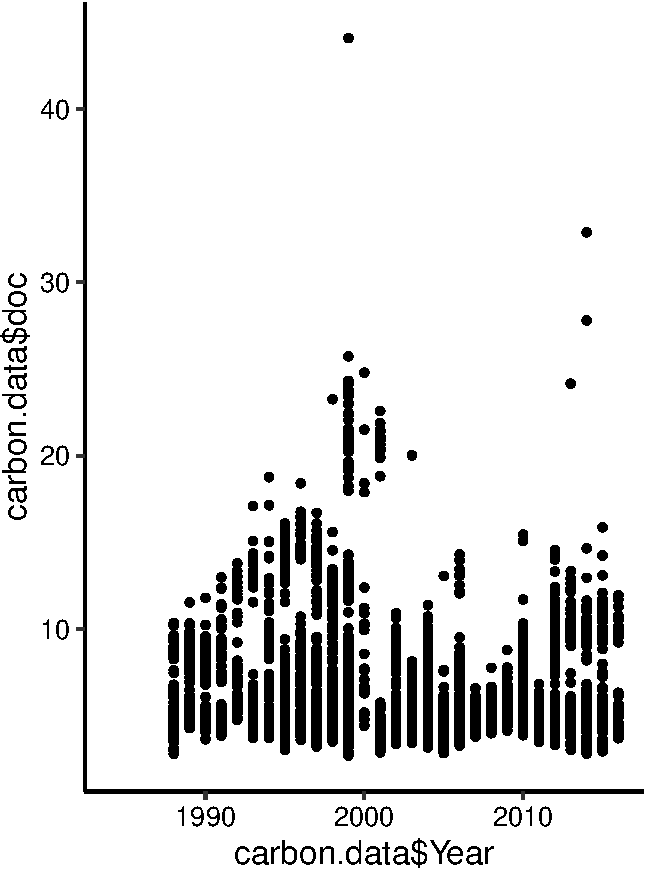
\includegraphics{Watson_ENV872_Project_files/figure-latex/unnamed-chunk-3-1.pdf}
\caption{\label{fig:fig1}Dissolved Organic Carbon (DOC) over time}
\end{figure}

The following graphs explore the Carbon dataset. \autoref{fig:fig1}
shows dissolved organic carbon over time. \autoref{fig:fig1} was created
to determine if there was a pattern of dissolved organic carbon in lakes
over the years. \autoref{fig:fig2} is a frequency polygon graph looking
at the dissolved inorganic carbon (DIC) in each lake. This graph was
created to see if there are some lakes with higher DIC than others,
which could influence further analysis.

\begin{Shaded}
\begin{Highlighting}[]
\CommentTok{#frequency polygon graph looking at DIC in each lake}
\KeywordTok{ggplot}\NormalTok{(carbon.data) }\OperatorTok{+}\StringTok{ }
\StringTok{  }\KeywordTok{geom_freqpoly}\NormalTok{(}\KeywordTok{aes}\NormalTok{(}\DataTypeTok{x =}\NormalTok{ carbon.data}\OperatorTok{$}\NormalTok{DIC_mg, }
                 \DataTypeTok{color =}\NormalTok{ Lake.Name), }\DataTypeTok{bins =} \DecValTok{20}\NormalTok{)}
\end{Highlighting}
\end{Shaded}

\begin{figure}
\centering
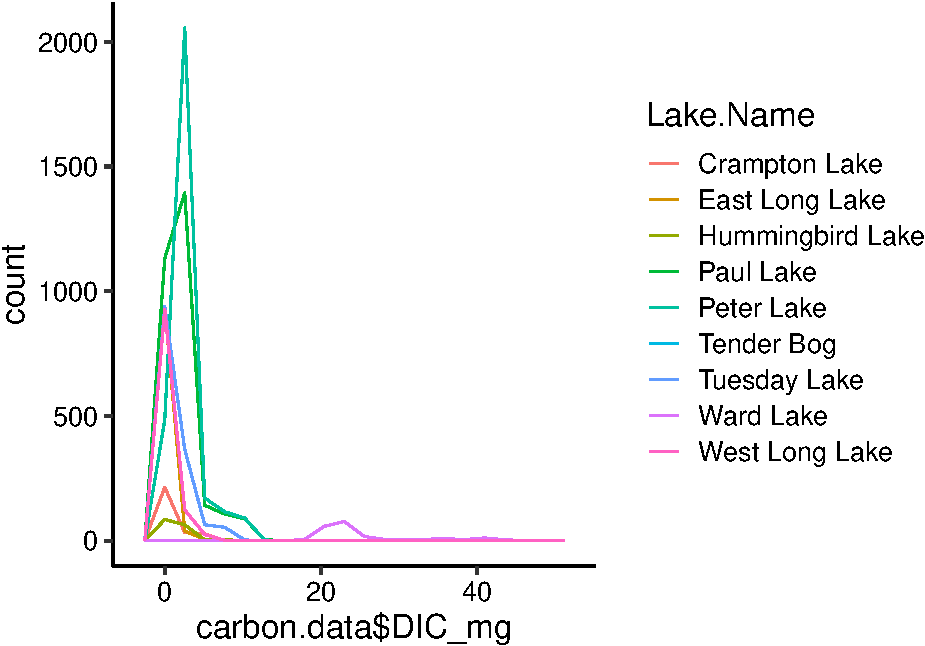
\includegraphics{Watson_ENV872_Project_files/figure-latex/unnamed-chunk-4-1.pdf}
\caption{\label{fig:fig2}Dissolved Inorganic Carbon in each Lake}
\end{figure}

\begin{Shaded}
\begin{Highlighting}[]
\CommentTok{#}
\end{Highlighting}
\end{Shaded}

\begin{Shaded}
\begin{Highlighting}[]
\CommentTok{#selecting date, DIC, DOC, Lake Name}
\end{Highlighting}
\end{Shaded}

\newpage

\section{Analysis}\label{analysis}

\newpage

\section{Summary and Conclusions}\label{summary-and-conclusions}


\end{document}
